\noindent
\begin{minipage}[t]{0.11\textwidth}
  \vspace{0pt}
  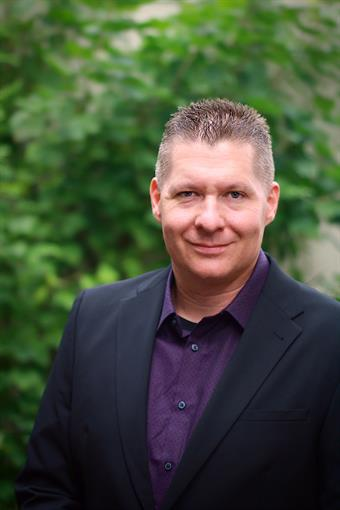
\includegraphics[width=\linewidth]{figures/portrait.jpg}
\end{minipage}\hfill
\begin{minipage}[t]{0.85\textwidth}
  \vspace{0pt}
  Dennis Müller is Professor of Artificial Intelligence at Hochschule
  Düsseldorf, Faculty of Media. His teaching focuses on artificial
  intelligence, machine learning, mathematics, and programming. In his
  courses, he places particular emphasis on understanding the principles
  behind modern AI systems, critically evaluating technological choices,
  and connecting technical methods with their broader societal and practical
  context. He initiated the KI-Con as a format in which students can present,
  discuss, and reflect on their own AI projects beyond the traditional
  classroom setting.
\end{minipage}
